\section{Bài 1:}
\begin{enumerate}
\bf
\item Sử dụng mô hình cho sẵn (đính kèm trong tập tin Project3{\_}1.pkt) để trả lời các yêu cầu bên dưới:

\rm Điền thông tin còn thiếu vào bảng: (các ô không có dấu -):
\begin{center}
\begin{tabular}{|c|c|c|c|c|}
\hline
\textbf{Device}&\textbf{Interface}&\textbf{IP address}&\textbf{Subnet mask}&\textbf{Default gateway}\\
\hline
Router0&G0/0&192.168.1.1&255.255.255.0&-\\
\hline
Router0&G0/1&192.168.8.1&255.255.255.0&-\\
\hline
Router1&G1/0&192.168.2.1&255.255.255.0&-\\
\hline
Router1&G1/1&192.168.8.2&255.255.255.0&-\\
\hline
PC0 (PC1 trên hình \ref{fig1.1})&-&192.168.1.10&255.255.255.0&192.168.1.1\\
\hline
PC1 (PC2 trên hình \ref{fig1.1})&-&192.168.2.10&255.255.255.0&192.168.2.1\\
\hline
\end{tabular}
\end{center}
\begin{figure}[H]
\begin{center}
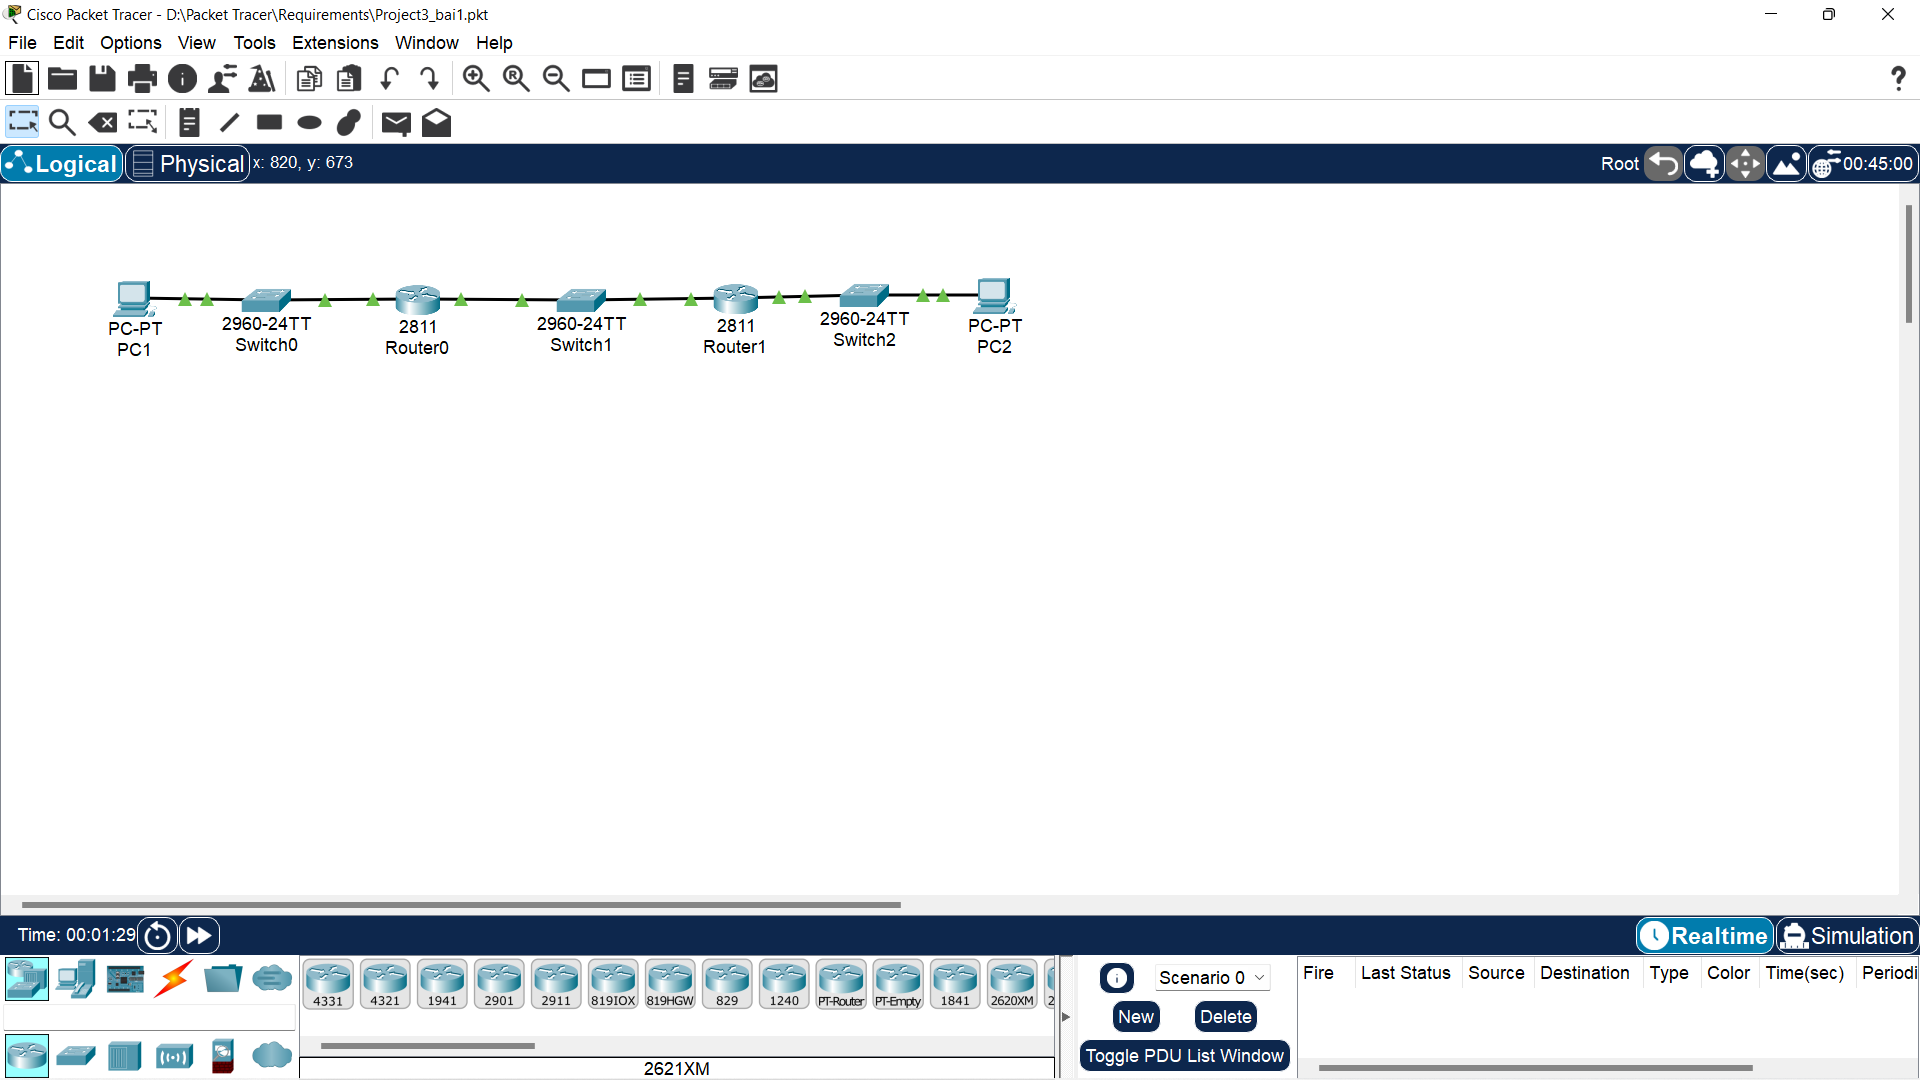
\includegraphics[scale=0.4]{../figures/p1/p1-prob}
\end{center}
\caption{Nội dung tập tin Project3{\_}1.pkt ban đầu}
\label{fig1.1}
\end{figure}

\begin{figure}[H]
\begin{center}
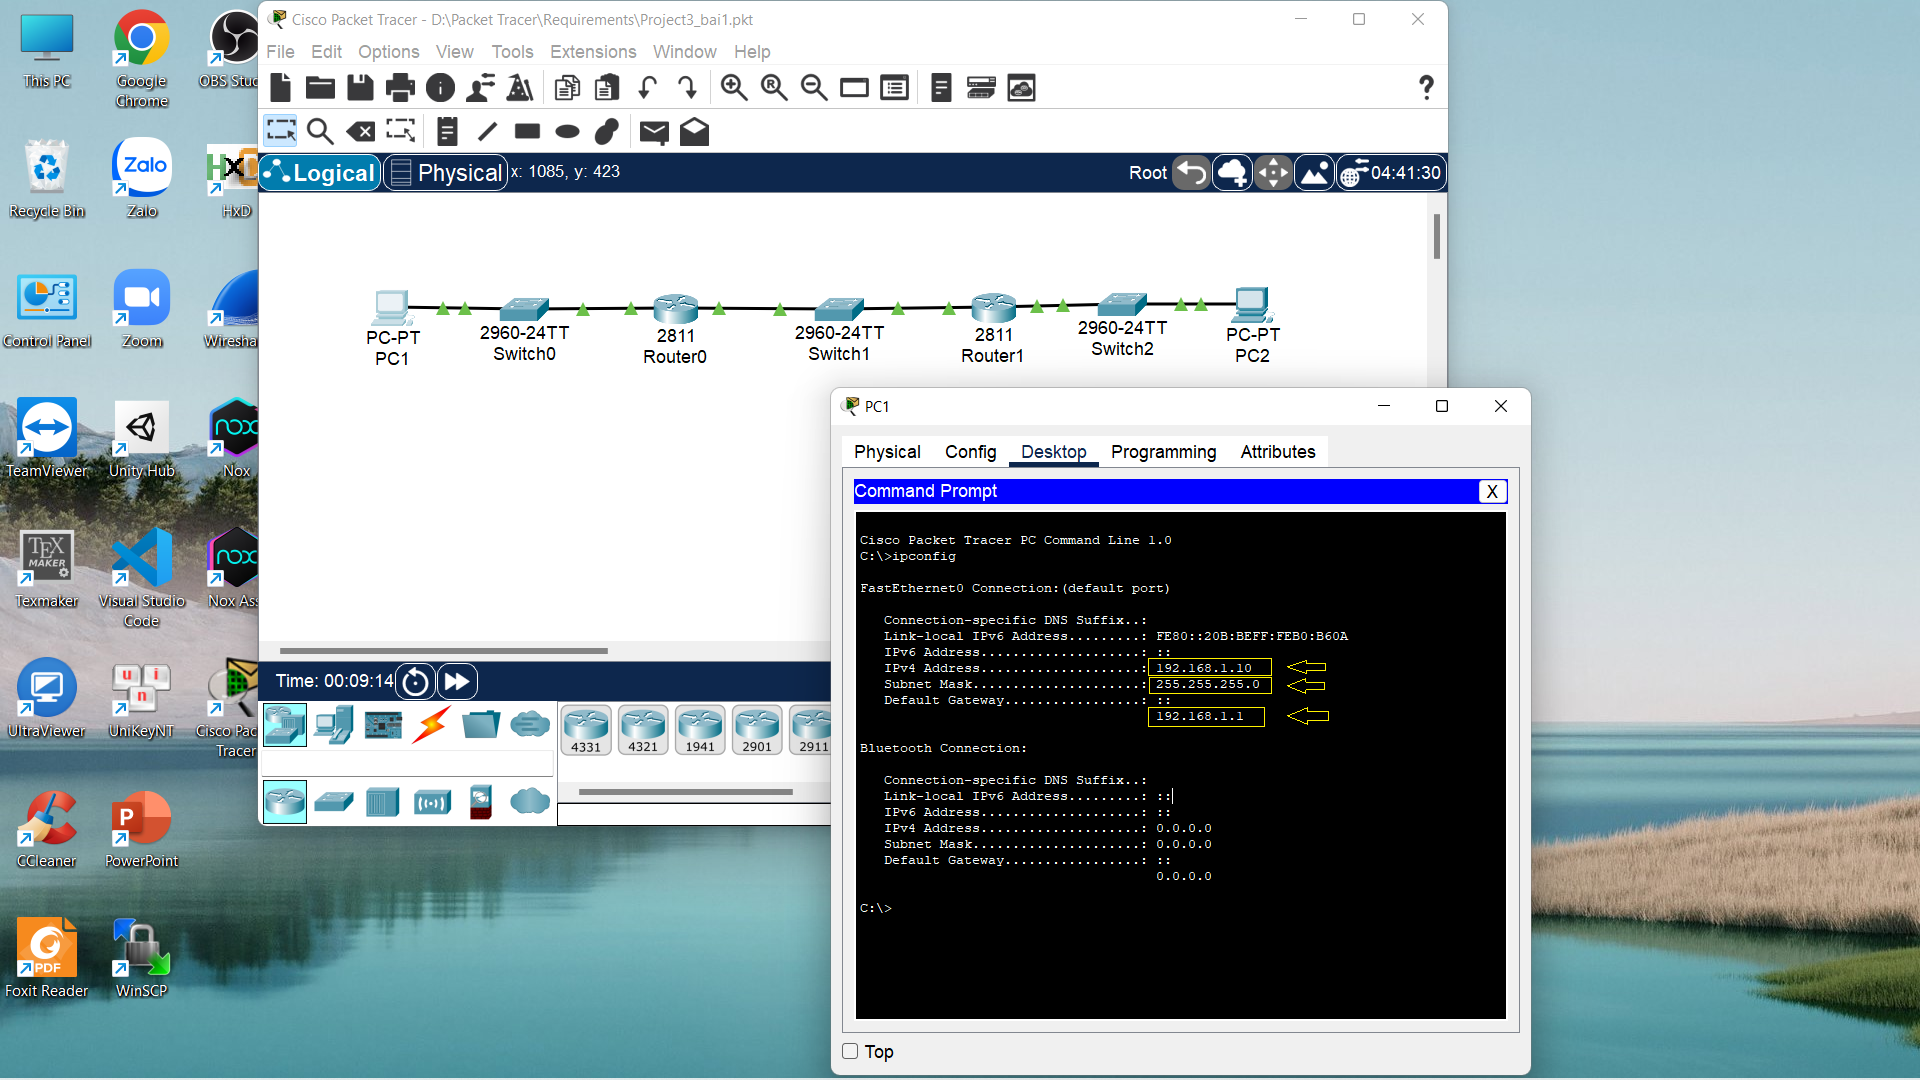
\includegraphics[scale=0.4]{../figures/p1/p1-ipconfig-pc}
\end{center}
\caption{Kiểm tra thông tin IP của PC}
\end{figure}

\begin{figure}[H]
\begin{center}
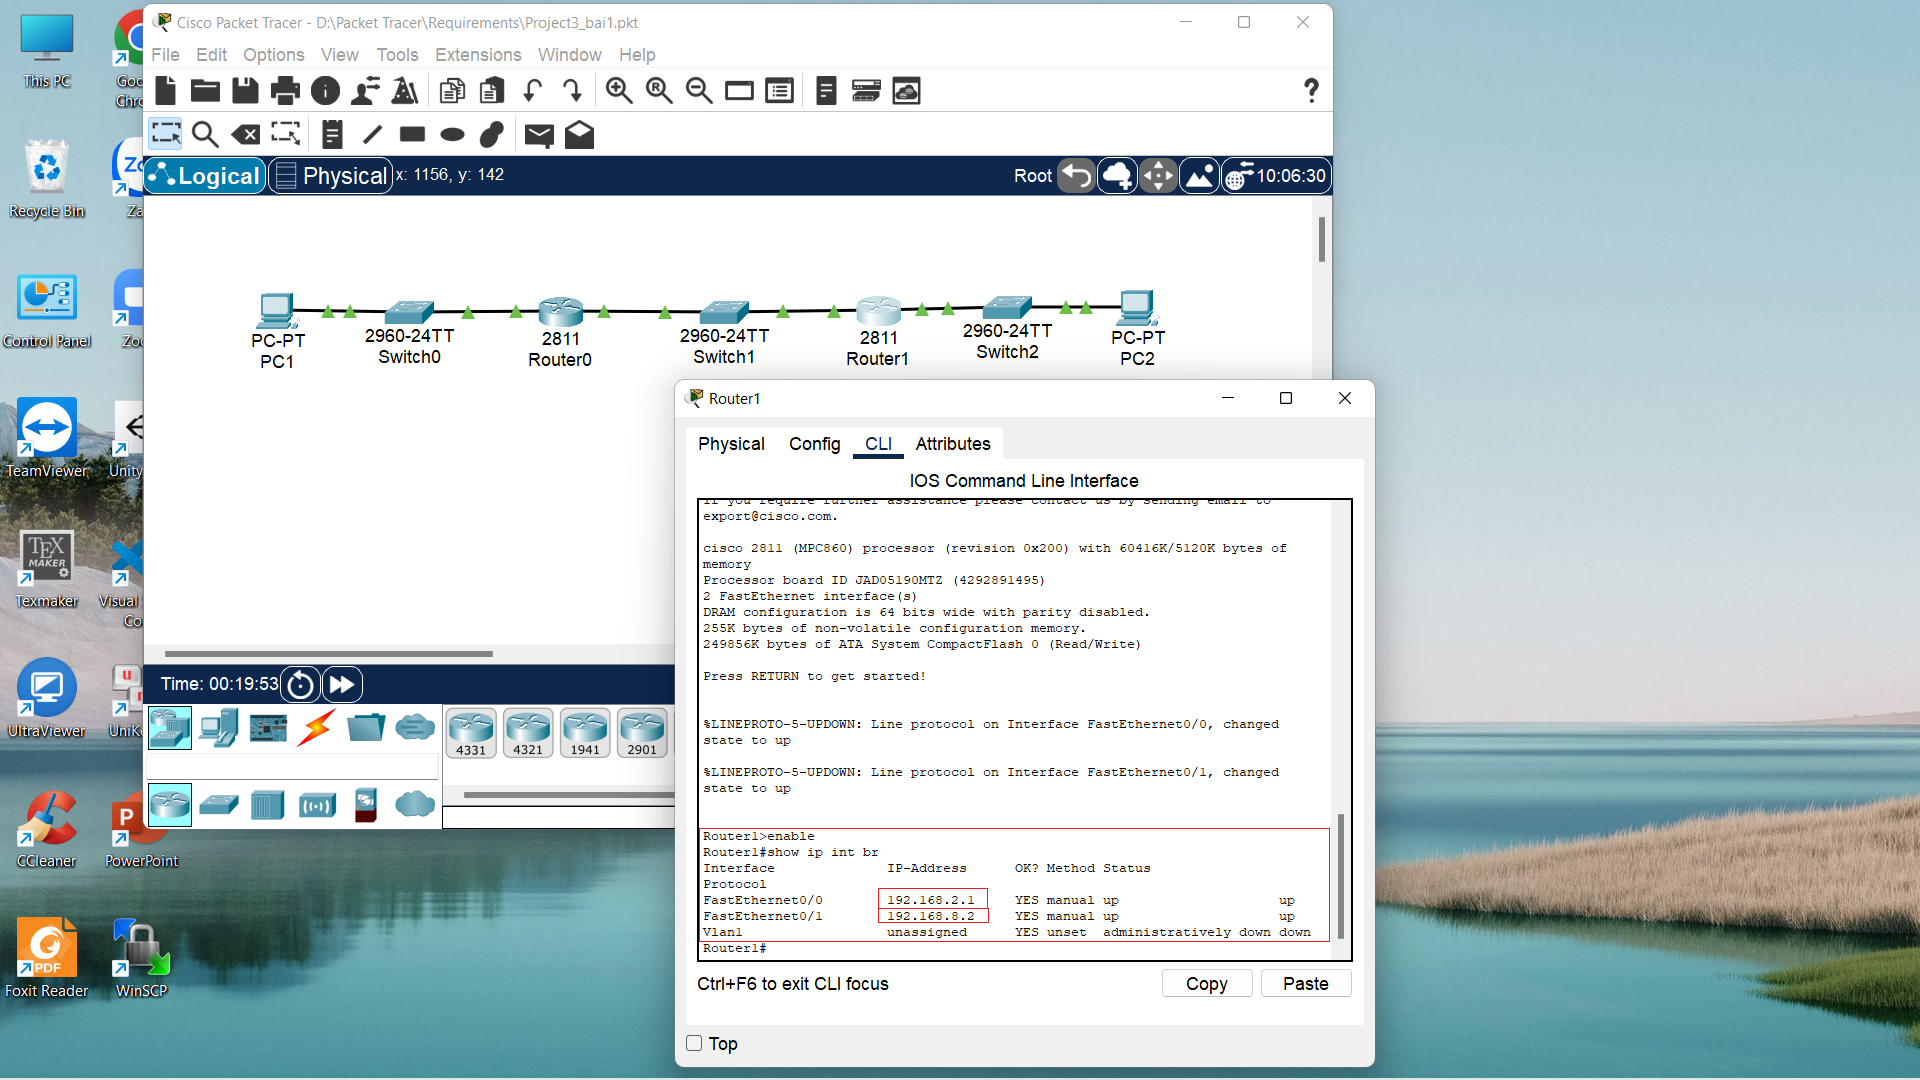
\includegraphics[scale=0.4]{../figures/p1/p1-ipconfig-router}
\end{center}
\caption{Kiểm tra thông tin IP của router}
\end{figure}

\bf \item Ghi chú đầy đủ các thông tin interface, địa chỉ đường mạng, địa chỉ IP lên mô hình mạng:

\rm 

\bf \item Ghi chú đầy đủ các thông tin interface, địa chỉ đường mạng, địa chỉ IP lên mô hình mạng:

\rm

\bf \item Kiểm tra kết nối từ PC0 đến PC1, cho biết kết quả như thế nào? (ở lần ping đầu tiên các gói tin icmp có được gửi thành công hay không). Cho biết đường đi của gói tin icmp (đi qua các thiết bị, IP nào?)

\rm

\bf \item Thêm PC2 vào đường mạng 192.168.8.0/24. Cấu hình địa chỉ IP, subnetmask, gateway tương ứng cho PC2.

\rm

\bf \item Kiểm tra kết nối từ PC0 đến PC2, cho biết kết quả như thế nào? (ở lần ping đầu tiên các gói tin icmp có được gửi thành công hay không). Cho biết đường đi của gói tin icmp (đi qua các thiết bị, IP nào?)

\rm

\bf \item Thay thế đường default route có trong Router0, Router1 bằng cấu hình định tuyến tĩnh sao cho tất cả các subnet có trong mô hình có thể kết nối lẫn nhau.

\rm

\bf \item Kiểm tra kết nối tất cả các subnet trong mô hình.
\end{enumerate}
